\chapter{Problem description}\label{ch:problem_desc}
% News & generic usage
While mobile devices have become ubiquitous and powerful for spreading digital information quickly, present-day commercial services and centralized infrastructure pose risks with regard to freedom and privacy.
In this chapter, these risks are discussed in more detail, we explain how fully decentralized distributed solutions can help to increase resilience, and we present the contributions of this thesis.

\section{Privacy and censorship}
%% Censorship
Pervasive monitoring of digital citizens by Internet providers on behalf of governments to enforce censorship laws raises severe privacy concerns \cite{nsa_privacy}.
% Large scale monitoring
The lack of anonymity becomes a problem when the users privacy is being invaded.
Revealing personal information can be deduced from search queries for example, or associations on social platforms.
When this information can be used for targeted advertising it becomes very valuable, and creates an incentive for the parties that have access to this information to sell it to third parties.
%% Invasion of privacy
Social media companies use targeted advertisement as part of their business model.
Information considered private by users of social media is actually used to broker targeted advertisements.
Subsequently users can be confronted with their information being misused in various ways beyond their control.
This lack of control over your own privacy can lead to arbitrary interference as defined in UDHR article 12. %ref, example, human rights watch, nelie kroes, etc.
Integration of social media on regular websites makes every page-view and click on these websites traceable to an individual, directly benefiting the business model of targeted advertisements
In fact the business model of social media appears to be serving targeted advertisements to its users on behalf of third parties.
Even more risk for violation of privacy, comes from integrating social media into regular websites, to de-anonymize and track the whereabouts of users even outside of the realm of social media.
Whenever users lose control over their privacy it becomes a serious problem.

% Dissent
The incentive to de-anonymize the user, not only causes a lack of privacy, but also a potential lack of freedom of expression, as it hands key information to a censor: who is expressing dissent and who is associated with this person on-line.
Cyber-suppression has become a reality when you no longer can be associated with opinion-makers or foreign journalists on-line.

% Single point of entry
Internet exchange (IX) infrastructures are among the central components in the inter-network architecture that are also vulnerable to monitoring, censorship and Internet kill-switches.
As such, not everyone has unrestricted access to the Internet due to censorship and surveillance.
In fact a significant part of today's Internet users is affected by these attempts to hide or distort reality. %ref
This interference directly affects the universal right to freedom of opinion and expression as stated in article 19 of the Universal Declaration of Human Rights (UDHR).

Cuba offline Internet \cite{watts2014havana}.
For example: Arab Spring, kill switches are real \cite{renesys2011egypt}, within half an hour all networks were unreachable. Syrian offline \cite{renesys2012syria}.
China: Apple's news app deactivated \cite{nyt2015appleChina}, last year. Censorship in China \cite{hrw2006china}.
BBC: China and Iran \cite{kathuria2010bypassing}. Censorship in Iran \cite{halderman2013iran}.
Turkey social media block \cite{twitter2015turkey}.

What are kill-switches?


Large portions of the global dialog on social media is uncontrolled by traditional media or governments.

Utilizing infrastructure is undesired because of censorship.


The sophistication of censorship techniques is pushed forward by the drive to stay ahead of attempts trying to circumvent it.
Increasingly though, Internet traffic is put under surveillance and obfuscation techniques are targeted by restrictions.


\section{Adversary model}\label{sec:adversary_model}
From the Arab Spring scenario we know Internet kill switches are real, so we must assume the existence of a powerful adversary.
The following threats \cite{ietf-shadow-internet} have been identified for similar circumstances:

\begin{itemize}
\item{
	The adversary can observe, block, delay, replay, and modify traffic on the underlying network.
	Thus end-to-end security must not rely on the security of the underlying network.
}
%\item{
%	Wireless communication is regularly monitored.
%	Responding to any wireless requests from a stranger is a direct threat to the user and extremely harmful.
%}
%\item{
%	Possession of encrypted electronic messages or encryption technology in general is extremely harmful to the smartphone owner.
%}
\item{
	The adversary has a limited ability to compromise smartphones or other participating devices.
	If a device is compromised, the adversary can access any information held in the device's volatile memory or persistent storage.
}
\item{
	The adversary can choose the data written to the transport layer by higher protocol layers.
}
\item{
	The adversary cannot break standard cryptographic primitives, such as block ciphers and message-authentication codes.
}
\end{itemize}
%Encryption is not a sufficient requirement of the friend-to-friend scenario, everything MUST be hidden.
%Possession of smartphones apps with encryption is already dangerous for the owner.
We assume the adversary cannot eavesdrop, jam, delay, replay, modify or spoof wireless communication between smartphones.
The adversary cannot compromise smartphones or other participating devices.
%Sybil?

\begin{figure}[H]
	\centering
	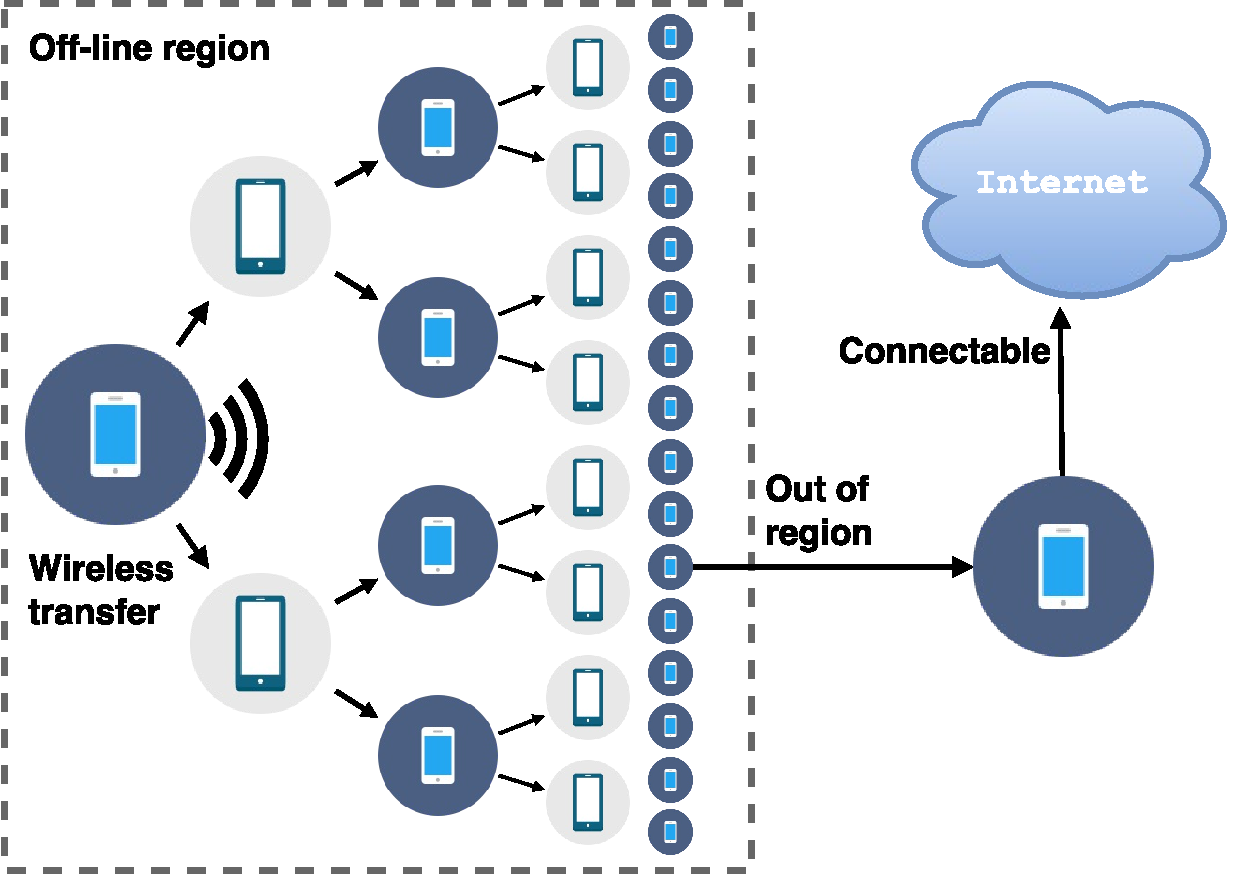
\includegraphics[width=0.7\textwidth]{viral_spreading}
	\caption{Viral spreading from one device to another within an off-line region}
	\label{fig:viral_spreading}
\end{figure}

\section{Distributed solutions}\label{sec:distributed_solutions}
%TODO: van een algemene naar specifieke case:
%- fully distributed oplossingen geven meer resilience tegen kill switches etc
%- mobiele oplossingen geven nog meer resiliency en zijn dus belangrijk om mogelijk te maken
%- zie plaatje: er is nog geen bruikbare oplossing
%- Tribler is een fully distributed systeem ontwikkeld op TUD
%- we gaan nu Tribler op mobiel mogelijk maken. Van "the only way to take Tribler down is to take the Internet down" naar "the only way...take everybody's smartphones away"

To ensure that no controlling party can exercise censorship authority must be distributed over all users. % creating an \emph{autonomous} system.
If all information is located in one or a few places, the parties in charge of that location will still have control over it, so information must distributed all users as well, creating a \emph{communication} system.
Finally, all users must be able to share, order and appreciate information of other users, in other words the essence of social media: social interaction.
With everyone being able to interact in the same way we need to  distribute functionality over all users, creating a \emph{cooperation} system.
% Solution
Fully distributed systems capture the characteristics just mentioned.
To render the effect mute of the Internet kill switches in existence shown to be used we propose a distributed solution.
Without any central component in the system it is no longer susceptible to censorship without everyone participating.
Leveraging the properties of mobile devices, like smartphones as stated above, together with the features of Tribler we see a perfect match.
Because censorship and large scale monitoring is difficult in decentralized networks our proposed solution can work in these situations.

% Eindig aantal servers points of failures
Networks that are not fully decentralized can be disrupted by taking down a limited number of nodes, less than the total number of nodes.
Thanks to a server-less design we can say:
The only way to take Tribler down is to take the entire Internet down.

\begin{figure}[ht]
	\centering
	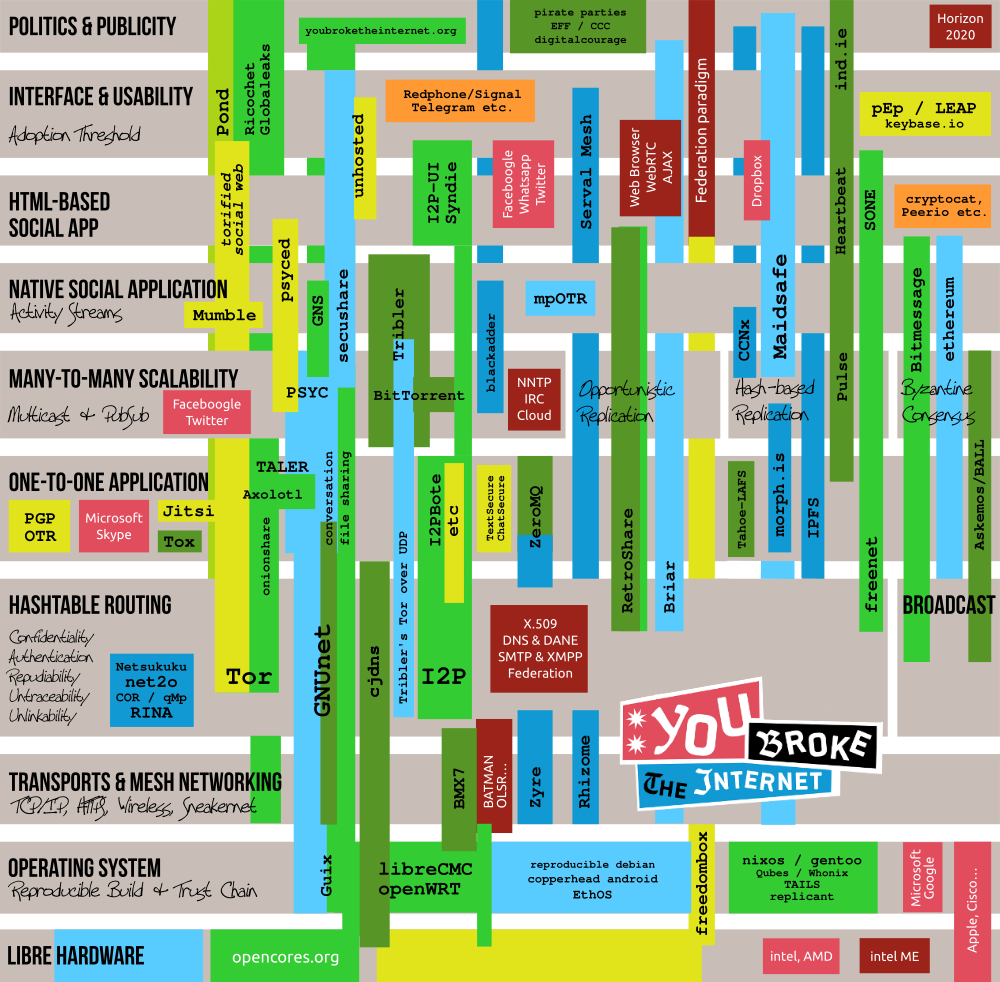
\includegraphics[width=\textwidth]{youbroketheinternet}
	\caption{Various partial solutions to mend the broken Internet according to www.youbroketheinternet.org}
	\label{fig:youbroketheinternet}
\end{figure}

The following network properties are defined \cite{hasan2013dissent} to provide a technical solution that enables free expression in the face of an adversary as defined in Section \ref{sec:adversary_model}:
\begin{itemize}
	\item \emph{Resilient against communications blackouts.}
	Should be challenging for any entity to disable.
	\item \emph{Resistant to monitoring and tracking of users.}
	Both who is using the network and any sensitive messages they send should be secret.
	\item \emph{Able to be built from innocuous components.}
	Should only require readily available hardware, and the possession and use of required hardware should not be illegal or suspicious.
	\item \emph{Able to run at meaningful scales.}
	Should be more effective at disseminating information than people with megaphones; more broadly, given a level of service, should be able to run at non-trivial scales.
\end{itemize}

Mobile devices are essential to take the next step in the face of censorship.
If we can use smartphones to create a fully decentralized social network we can say:
The only way to take Tribler down is to take everybody's smartphones away.

The importance of mobile devices in this context is crucial, if we want to do even better in spreading information, which is not been done before, we surmount than next hurdle.

Peer-to-peer communication technology is essential for a server-less distributed system.
Mobile devices typically do not require infrastructure to exchange information, like those equipped with Bluetooth or capable of ad hoc Wi-Fi.
Smartphones are ubiquitous everywhere in the world and used to access social media and retrieve information from the Internet.
Fortuitously these are also the type of mobile devices that can communicate peer-to-peer.

Example: Arab spring \cite{pouwelse2012censorshipfree}


% Fragmented
Various initiatives have been started to deal with one or both of these problems \cite{redecentralize2015alternativeinternet}.
%FIG? From re-decentralized: top projects that match/compare.

Figure \ref{fig:youbroketheinternet} shows a mapping of projects that are or have been working on that.
The fragmentation is clear from the figure.
There are a few big players, as can be seen from the figure, but none of them provide a full solution.

%potential skip:
%being first
%engineering perfection
%time to market
%popularity
%make a difference
%Tribler mobile vs periscope
%fully functional prototype, but poor user interface (unpolished)
%real world impact proven insufficient
%we want to change the world implicit


%\section{Define alternatives} %design space %solution space
%\cite{https://www.ietf.org/mail-archive/web/ietf-privacy/current/msg00215.html}
% why existing technology is not sufficient to
% meet the described demands. The example proposed was the tor onion
% network in combination with XMPP or the orbot smartphone app. After
% much discussion the conclusion was that existing technologies, such as
% tor facilitate protected point-to-point communication. However,
% possible desired use cases focus more on current Twitter-like social
% media practices, best typified as a "global conversation".
% Furthermore, current social media revolves around video-rich,
% real-time interaction with groups, hashtag-based discovery and social
% networking. All of these aspects are not offered or are incompatible
% with current-generation of privacy enhancing technology



% Refereren aan eigen werk versplintering in oplossingen
There is no de-facto solution available on mobile platforms. \cite{literature_survey}
Previous research has shown that there is no solution that solves the problem entirely in a sustainable way.
Tribler is our attempt to solve this problem entirely in a sustainable way.
To see if it is feasible to apply it in a mobile context as described above, we need to port it.


\section{Contributions}
The main contribution of this thesis is making Tribler available on mobile devices and the utilization of their unique properties in the context of censorship and communication during crises.
This work also enables a new direction for future research with Tribler: mobile devices.
The resilience of Tribler against attacks on the Internet is greatly increased.
The goal of Tribler is to become an information sharing platform that protects the privacy of its users and is resilient to attacks while not relying on existing infrastructure.

% Previous Tribler-mobile app's
Previous attempts did not to deliver all functionality \cite{tribler2014play,tribler2014at3,tribler-anon-hd}.
Maintainability issues with earlier designs, and large amounts of technical debt \cite{thesis_martijn}, were the major causes.
We changed the architecture of Tribler for our approach.

The scientific contributions of this work are the experiments to verify the feasibility of Tribler on mobile devices and the ability to perform research with Tribler fully geared towards mobile devices


